\subsection{Tradeoff analyzed: training resources - model accuracy}\label{sec:experiments:exp1}

\begin{table}[t]
\centering
\caption{Model training performance. TT = training time, MPD = mean power draw.}
\label{tab:eval:power-stuff}
\begin{tabularx}{\linewidth} {XXXX}
    \toprule
    Model & MPD [W] & TT [h] & Accuracy \\
    \midrule
    SiMo  & 155              & 6.70              & 34.37\%             \\
CoMo  & -         & 36.65          & 57.80\%             \\
b0    & 178              & 6.36              & 55.31\%             \\
b1    & 185              & 8.70              & 53.70\%             \\
b2    & 187              & 9.34              & 54.63\%             \\
b3    & 183              & 12.25             & 51.41\%    \\
    \bottomrule
\end{tabularx}
\end{table}

As with many complex classification tasks, object classification presents itself with an inherent trade-off between training costs and model accuracy \cite{DBLP:conf/icml/TanL19}. Inherently, models of increasing complexity pose a challenge to fulfilling the requirement of live and instantaneous predictions \ref{nfr1}. While intricate models (e.g., CoMo), employ multiple components to enhance accuracy, they often require significantly more computational resources in contrast to simpler models such as SiMo. These models demand less computational efficiency but potentially compromise accuracy \ref{nfr2}. Prior work shows that, while ensemble-like models can improve generalization \cite{DBLP:journals/ml/Dietterich00}, their efficiency-to-performance ratio is not always optimal, making model selection a crucial factor in balancing accuracy and computational cost.

With this experiment, we quantify this trade-off by analyzing the relationship between GPU power usage (wattage) and accuracy across five different models: EfficientNet-B0, B1, B2, and B3 components of CoMo, and our SiMo architecture.  For this experiment, we tracked two key metrics during the training process: model performance as final accuracy and training costs as GPU power consumption over time.

The data gathered (\Cref{tab:eval:power-stuff}) from measuring GPU power consumption revealed important efficiency trade-offs. While SiMo had the lowest power draw of 155W, its accuracy (34.4\%) lagged behind all EfficientNet models.

Surprisingly, EfficientNet-B0 boasted the second-highest accuracy (55.3\%) at the second-lowest power draw of 178W \ref{nfr5}, \ref{nfr2}, outperforming B3, which consumed 3\% more energy for nearly twice as long, yet achieving 7\% lower accuracy.

\Cref{fig:exp1:fig6} shows the accuracy per watt for each model. SiMo demonstrates the lowest accuracy-to-efficiency ratio of 0.22\%/W, reflecting its design prioritization of computational resources over performance. Out of all EfficientNets \ref{nfr3}, we identify that B0 yields the best performance-per-energy ratio, with 0.31\%/W. These results demonstrate that larger models do not necessarily guarantee better performance. \Cref{fig:experiment:power-costs} additionally demonstrates GPU power consumption over time for training each model. The total energy consumed is significantly higher for EfficientNets of larger complexity.

\begin{figure}
    \centering
    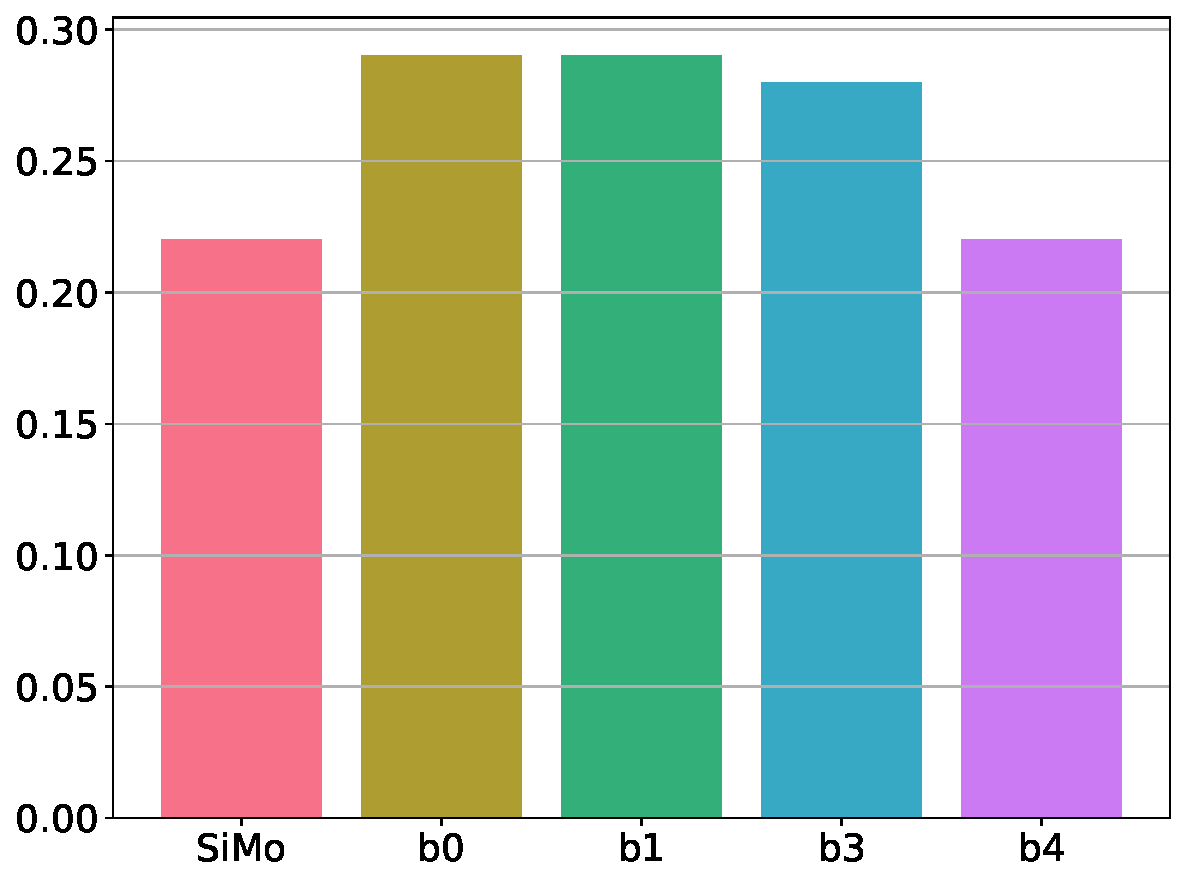
\includegraphics[width=1\linewidth]{figures/accuracy_per_watt.pdf}
    \caption{Accuracy Per Watt.}
    \label{fig:exp1:fig6}
\end{figure}

CoMo’s architecture design proved greedy, consuming around five times more energy than its highest-performing component (EfficientNet-B0) \ref{nfr5} while delivering only a slightly higher accuracy of 57.8\%. The aggregate training costs of 734 watts and 36.6 hours reveal severe inefficiencies when examined next to the underwhelming gains in accuracy compared to simply using one of its component models. This finding demonstrates that a tradeoff between model architectural complexity and model training costs in low-resource environments \ref{nfr5} results in smaller models. CoMo, as its aggregated training cost significantly outweighs its marginal performance benefits. While the theoretical advantage of integrating multiple EfficientNet models suggests enhanced feature extraction and generalization, our results indicate that the efficiency-to-performance trade-off does not justify the increased resource consumption. In particular, EfficientNet-B0 emerges as a notably strong performer, fully adheres to high accuracy requirement \ref{nfr2} with significantly reduced energy demands compared to larger models and the full CoMo architecture.

A main finding from this experiment is that larger, more complex models do not inherently guarantee superior results \ref{nfr2}. Instead, the computational cost must be weighed against the actual gains in accuracy. In this case, CoMo’s inability to significantly outperform its own component models highlights inefficiencies in its design. Future work should investigate whether alternative integration strategies or architectural optimizations could improve the efficiency of this approach, and especially whether different combinations of component models could offer different advantages.
% Additionally, while our analysis shows that a single well-selected model (EfficientNet-B0) can rival more elaborate architectures,
Other complex approaches, designed with more effective fusion strategies or optimized training methodologies, could yield superior performance without incurring excessive computational costs. Exploring these alternative architectures, such as weighted ensembling techniques, dynamic model selection, or adaptive training schedules, could provide insights into achieving a better balance between accuracy and efficiency in large-scale classification tasks.

Overall, our findings suggest that when designing classification models, considerations of training cost and efficiency should be given equal weight alongside performance. This perspective can help inform future research directions, guiding efforts to develop high-performing models that also maintain sustainable computational demands.





% % \usepackage{tabularray}
% \begin{table}
% \centering
% \begin{tblr}{}
% Model & Mean power draw (W) & Time to train (h) & Accuracy          \\
% SiMo  & 155              & 6.70              & 34.37\%             \\
% CoMo  & see b0-3         & see b0-3          & 57.80\%             \\
% b0    & 178              & 6.36              & 55.31\%             \\
% b1    & 185              & 8.70              & 53.70\%             \\
% b2    & 187              & 9.34              & 54.63\%             \\
% b3    & 183              & 12.25             & 51.41\%             
% \end{tblr}
% \end{table}





%Also we need to mention probs in section 4d that we didn't train to the fullest, and here that the accuracy is after training but knowing baselines (efficientnets trained on imagenet) we know that these models can achieve the accuracy of more than 80 percent) But also if we trained till it plateud maybe we fucked something up

\begin{figure*}
    \centering
    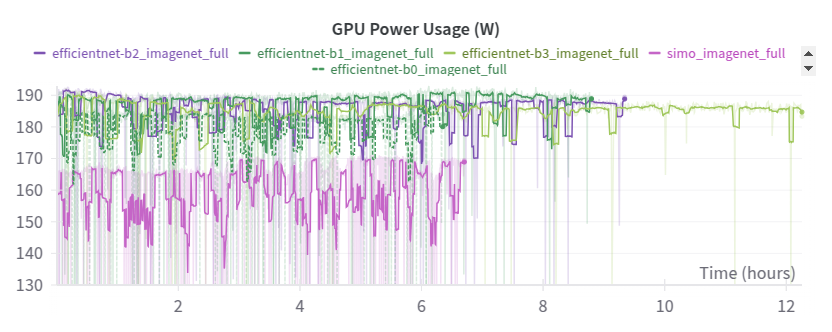
\includegraphics[width=0.95\linewidth]{figures/wattage-graph.png}
    \vspace{-0.3cm}
    \caption{Power costs for model training over time. We provide details for EfficientNet B0, B1, B2, B3, and SiMo.}
    \label{fig:experiment:power-costs}
\end{figure*}

